\documentclass{article}

% InterpScience (NeurIPS 2026) LONG track, CAMERA-READY: 9pp + refs/appendices.
% Accepted 2026-09-29. The anonymous submission as uploaded is the git tag
% `interpscience-submission` (commit b86a100); this file supersedes it and
% writeup_interpscience_deanon.tex. Run scripts/check_everything.sh after any edit.
\usepackage[final]{neurips_workshop}
\usepackage[utf8]{inputenc}
\usepackage[T1]{fontenc}
\usepackage{hyperref}
\usepackage{url}
\usepackage{booktabs}
\usepackage{amsmath,amssymb}
\usepackage{microtype}
\usepackage{graphicx}
\usepackage{enumitem}
% Coloured links print as black text and read better on screen than boxes.
\hypersetup{colorlinks=true, linkcolor=[rgb]{0.10,0.25,0.55}, citecolor=[rgb]{0.10,0.25,0.55}, urlcolor=[rgb]{0.10,0.25,0.55},
  pdftitle={What Happens to a Monitor's Accuracy When You Train Against It},
  pdfauthor={Abraham Yeung and Anagha Ramaswamy}}
% The bundled style's [final] notice names the main conference, not the
% workshop. Override it.
\makeatletter
\renewcommand{\@noticestring}{Interpretability as a Science (InterpScience) Workshop at NeurIPS 2026.}
\makeatother
\setlength{\abovecaptionskip}{4pt}\setlength{\belowcaptionskip}{0pt}
% No paragraph indents anywhere; vertical space separates paragraphs.
\setlength{\parindent}{0pt}\setlength{\parskip}{0.38em}
\setlength{\textfloatsep}{10pt}\setlength{\intextsep}{8pt}
% A page holding only floats starts them at the top rather than centring them.
\makeatletter\setlength{\@fptop}{0pt}\makeatother

\title{What Happens to a Monitor's Accuracy When You Train Against It}

\author{%
  Abraham Yeung\thanks{Correspondence: \texttt{ayeung16@stanford.edu}. Code and the regeneration script: \url{https://github.com/Abraham-y/reader-writer-probe-rl}.} \\
  Stanford University \\
  \And
  Anagha Ramaswamy \\
  Stanford University \\
}

\begin{document}
\maketitle

\begin{abstract}

A linear probe on a language model's hidden states predicts whether the model's next answer will be correct. On held-out prompts it ranks a correct answer above an incorrect one $98\%$ of the time. The probe we train against is a second fit of the same kind, on temperature-1 answers like those reinforcement learning samples. Used as the reward, it lowers true accuracy by $31$ percentage points.

The reward probe's AUROC does not show this for 30 to 40 training steps. Scored at every checkpoint on that checkpoint's fresh answers, it first falls at step 40, or first moves at step 50 if each answer is graded by its last answer block rather than its first, although task accuracy is already significantly lower at step 10. A frozen LLM judge that was never trained against ends the run with the AUROC it started with while accuracy falls from $54\%$ to $23\%$. A monitor's accuracy statistics describe the monitor together with the population it scores, and deploying the monitor is what moves the population. A stable AUROC says the monitor still separates correct answers from incorrect ones. It does not say how many answers are correct. The share of answers above a threshold frozen at the start moves without labels, by step 10 for the probe and by step 30 for the judge. For the probe that movement is partly guaranteed by the objective, and neither has been calibrated against matched benign training.

Held-out accuracy also did not rank our rewards by how safe they were to train against. Of three rewards trained under one recipe, the one that read lowest as a held-out monitor, a probe on activations with 39 surface features of the text regressed out (AUROC $0.834$), left the most accuracy ($0.168$). The same probe without that step ($0.978$) left $0.051$, and a monitor built only from those 39 text features ($0.925$) drove accuracy to exactly zero. The lowest-reading reward was also the weakest on the model it read during training, and it penalised the surface pattern rather than ignoring it, so this is a counterexample, not evidence that removing surface information makes a reward safe. Nothing in the objective rewards evading the monitor. The policy is doing what it was asked.

\end{abstract}

\section{Introduction}

A probe is a small classifier trained on a model's internal activations to predict some property of the model's behavior. Directions and detectors read from a model are increasingly used for more than analysis. Refusal directions steer behaviour when ablated or added \citep{arditi2024refusal}, truth probes aim to recover what a model knows apart from what it says \citep{burns2022discovering}, and lie detectors, black-box \citep{pacchiardi2023lie} or probe-based \citep{taufeeque2026atlas}, have been proposed as training signals. Placing a probe inside the training loop and optimizing against it is less well understood than evaluating the probe from outside the loop.

Reward overoptimization shows that optimizing too far against a learned proxy reward degrades the true objective, with no adversarial intent required \citep{gao2023scaling, coste2023reward}. Almost no non-trivial proxy is unhackable in principle \citep{skalse2022defining}, and gaming learned on easy targets can generalize to reward tampering \citep{denison2024sycophancy}. Monitor evasion shows that monitors of a model's chain of thought \citep{baker2025monitoring} or of its activations \citep{gupta2025rlobfuscation, bailey2024obfuscated} can be evaded when they are optimised against, though with enough KL regularisation and a strong enough probe penalty, training can instead yield honest policies \citep{taufeeque2026atlas}. Work on LLM evaluators reaches a related conclusion from the measurement side. Judges are usually validated by agreement with human labels \citep{zheng2023judging}, agreement statistics overstate how well they discriminate \citep{norman2026reliability} and hide their sensitivity to how the rubric is worded \citep{weng2026invariance}, and the measurement changes when the judge does \citep{yang2026auditing}. Reward-model benchmark scores track downstream outcomes unevenly, depending on the metric and on how the reward model is used \citep{frick2024ppe, malik2025rewardbench2}.

Both mechanisms are established. Less is known about what a monitor's own quality statistics do while the policy it scores degrades. \citet{baker2025monitoring} report that a chain-of-thought monitor's recall falls to near zero once the policy is optimised against it, measured against a programmatic check for one class of hack: whether the tests still pass once the agent's edits to them are reverted. They note that without such ground truth, one could not tell that the agent was misaligned. That case is evasion, because the monitor entered training as a penalty. In our setting the monitor enters as a positive reward, so there is nothing to evade, and Countdown provides exact ground truth for every answer at every checkpoint. This makes it possible to measure what a monitor's discrimination does while the policy is complying with it. In our run, the monitor's AUROC moves 30 to 40 steps after task accuracy. This is consistent with \citet{beigi2026prime}, who find that a policy's answers to direct questions about its proxy reward forecast later reward hacking while the visible hack rate is still low, and that activation directions for the same capability emerge before sustained hacking. The information exists, but it is not in the monitor's accuracy against its target.

This applies to probes in particular. Statistics such as AUROC and precision are not properties of a classifier alone. They are properties of a classifier together with a population, and the field reports probe AUROC as if it belonged to the probe. \citet{belinkov2022probing} argues that probe accuracy does not license the claim that the model uses the probed property. Probe accuracy also does not license a claim about the probe, because deploying the artifact changes the population on which the number was measured. The judge in \S\ref{sec:judge} is frozen. Its AUROC ends where it began, so it still discriminates, while the policy it scores loses most of its accuracy.

We work with Qwen2.5-0.5B trained on Countdown arithmetic \citep{gandhi2024stream} with RLOO \citep{ahmadian2024back}. The task has an exact verifier, so a learned scorer's divergence from ground truth can be measured directly, without confounds from preference modeling. Four different scorers are referred to in this paper as ``the monitor'', and the same checkpoints are sampled and graded under four protocols. Table~\ref{tab:actors} names each, and every figure and table below states which it uses.

\begin{table}[t]
\centering
\scriptsize
\setlength{\tabcolsep}{3pt}
\renewcommand{\arraystretch}{0.9}
\begin{tabular}{lllcl}
\toprule
\multicolumn{5}{l}{\emph{(a) the four monitors}} \\
name & what it reads & what it was fit to & AUROC & how it is used here \\
\midrule
trace-final probe & L16 \texttt{</think>} & headline answers, first block & $0.982$ & read-only; never a reward \\
reward probe & L16 \texttt{</think>}, \emph{another} fit & $T{=}1$ answers, last block & $0.810$ / $0.945$ & the RL reward; scored in Fig.~\ref{fig:lag} \\
surface model & 39 text features, no activations & headline answers, first block & $0.926$ / $0.925$ & free baseline; arm B's reward \\
LLM judge & \texttt{Qwen2.5-7B-Instruct} & not fit; a fixed prompt & $0.785$ & bystander; never optimised against \\
\midrule
\multicolumn{5}{l}{\emph{(b) the four evaluation protocols, all on the same 406 prompts, at most 1{,}024 new tokens}} \\
name & answers per prompt & sampling & block graded & where \\
\midrule
headline & 16 & $T{=}0.6$, top-$p$ 0.95, top-$k$ 20 & first & \S\ref{sec:probe-reader}; \S\ref{sec:probe-rl} accuracies \\
arm & 8 & $T{=}1$, top-$p$ 1 & first & arms A, B, R and C (Table~\ref{tab:arms}) \\
probe ladder & 8, fresh per checkpoint & $T{=}1$, top-$p$ 1 & both & \S\ref{sec:lag}, Fig.~\ref{fig:lag}, Tables~\ref{tab:lag},~\ref{tab:lagfirst} \\
judge ladder & 8, fresh per checkpoint & $T{=}1$, top-$p$ 1 & first & \S\ref{sec:judge}, Table~\ref{tab:judge} \\
\bottomrule
\end{tabular}
\caption{Who is who. \textbf{(a)} Where two AUROCs are given they are two fits of the same features under different label rules and splits, and are \emph{not} interchangeable: the reward probe reads $0.810$ on its own protocol (last block, on answers to 300 prompts from the RL training pool, none of them among the 406) and $0.945$ on the population the reward arms share (first block); the surface model reads $0.926$ under the \texttt{GroupKFold} of \S\ref{sec:probe-reader} and $0.925$ as the shipped arm-B artifact. Only the AUROC column of Table~\ref{tab:arms} is one common population, and it is the only held-out ranking; \S\ref{sec:surface} also reads arms A, B and R through $C_{\text{SFT}}$. \textbf{(b)} ``First block'' grades the first \texttt{<answer>} block in an answer, ``last block'' the last. During RL, sampling stopped at the first \texttt{</answer>}, so the verifier only ever graded the first block; every evaluation here samples without that stop, which is why later blocks exist at all. The two ladders are independent draws from the same checkpoints, and their first-block accuracies agree to within $0.016$ at every checkpoint. The headline protocol's settings are the sampler's defaults; its output files do not record them.}
\label{tab:actors}
\end{table}

\paragraph{Contributions.}
\begin{enumerate}[leftmargin=1.6em,itemsep=1pt,topsep=2pt]
  \item Held-out quality did not rank our monitors by how safe they were to train against. Our best monitor, the trace-final probe, reaches AUROC $0.982$. The probe trained against in our first runs is a second fit, on temperature-1 answers; it shares a direction with the first at cosine $0.192$, and it costs $31$\,pp when made the reward. The controlled comparison is between three rewards trained under one recipe and scored on one population. A probe on activations with surface features regressed out reads lowest as a held-out monitor ($0.834$) and left the most accuracy ($0.168$). The same probe without that step reads $0.978$ and left $0.051$, and a monitor built only from text features reads $0.925$ and drove accuracy to exactly $0.0000$ ($16.8$\,pp below the residualised probe, CI $[14.7, 19.0]$). The residualised probe's run ended $11.6$\,pp above the raw probe's (CI $[9.6, 13.8]$). Its reward was also the weakest on the model the arms read during training and penalised the surface pattern a text-only reward favours, so we do not attribute the gap to removing surface information. Single-seed runs give counterexamples, not a trend. (\S\ref{sec:probe-rl}, \S\ref{sec:surface})
  \item A monitor's AUROC did not detect the decline. Task accuracy on the probe-as-reward run is significantly lower by step 10. The reward probe's AUROC first falls at step 40 when answers are graded by their first block, the block the verifier graded during training, and first moves at step 50 when graded by the last block, the label the probe was fit to. Its likelihood ratio at a threshold frozen at step 0 falls sooner, by step 10, as inflating scores carry incorrect answers over the threshold faster than correct ones. The central case is a frozen LLM judge (fixed weights and prompt, greedy decoding) that was never optimised against. Over the run its AUROC and its likelihood ratio, which does not move with the share of correct answers, both end where they began. The judge still discriminates. Discrimination is a joint property of a classifier and a population, deploying the classifier is what moves the population, and a flat AUROC is compatible with a failing policy. The share of answers above a threshold frozen at step 0 registers the inflation at step 10, 30 to 40 steps before the AUROC moves, without labels. For the probe that early movement is partly guaranteed by the objective, and using the statistic as an alarm would require a matched benign control, which has not been run. (\S\ref{sec:lag}, \S\ref{sec:judge})
\end{enumerate}

\section{Setup}\label{sec:setup}

We use Qwen2.5-0.5B on Countdown. Given 3--4 integers and a target, the model must produce an equation using each integer exactly once, checked by an exact rule-based verifier. $C_{\text{SFT}}$ is a supervised checkpoint. $C_{\text{outcome}}$ is 100 RLOO steps against the verifier, which raises first-block accuracy on our 406 evaluation prompts from $0.290$ to $0.550$. The evaluation set is 406 procedurally generated problems with no overlap against the RLOO training pool. AUROC here is the probability that a randomly chosen correct answer scores above a randomly chosen incorrect one, so $0.5$ is chance. It is seed-dependent at the $\sim$0.015 level, and we do not rely on a third decimal. Appendix~\ref{app:setup} gives the probes, hyperparameters and estimator.

\section{The probe is a good detector}\label{sec:probe-reader}

A trace-final probe on layer-16 \texttt{</think>} states reaches AUROC $0.982$ on $C_{\text{outcome}}$'s headline answers, held out by prompt, meaning it is scored on prompts it was not fit on. As a best-of-16 selector it captures $88.8\%$ of the accuracy gain available to any selector (CI $[78.9\%, 96.5\%]$). Free baselines come close, which matters in \S\ref{sec:surface}. \texttt{</think>} position alone scores $0.915$, and a 39-feature surface model scores $0.926$. As a selector the probe beats both free baselines by $+3.20$\,pp of selection accuracy. The probe is a good detector that partly relies on a cheap surface correlate, and it is not only a length detector. Appendix~\ref{app:reader} gives the baselines and the length controls.

The probe evaluated here is not the probe trained against below, and the two share little direction (cosine $0.192$). To match the temperature-1 answers the policy samples during RL, rather than the trace-final probe's temperature-0.6 answers, the reward probe was fit separately, on temperature-1 answers to 300 prompts from the RL training pool. None of those prompts is among the 406 evaluation prompts. Its labels grade the last answer block of answers sampled without the stop at \texttt{</answer>} that RL training used, and its held-out AUROC on that protocol is $0.810$. On $C_{\text{outcome}}$'s headline answers graded by the first block it reads $0.951$. The reward probe is also the probe scored at every checkpoint in \S\ref{sec:lag}, under both labels. The separate fit was a choice, not a requirement: arm R of \S\ref{sec:surface} trains against a probe fit on temperature-0.6 answers, at cosine $0.779$ with the trace-final probe.

\section{Using the probe as the reward destroys the task}\label{sec:probe-rl}

The reward probe is now the quantity the model is trained to maximize. The reward is its $P(\text{correct})$ at \texttt{</think>}, read from the current policy's hidden state; the probe is fixed, and the copy of the policy it reads is refreshed each round (except on one round in ten, Appendix~\ref{app:setup}). The verifier still runs, but only to log true accuracy. It does not enter the gradient. Training runs 100 RLOO steps with the vanilla run's learning rate, KL and entropy coefficients and sampling, but with group size 8 rather than 16, weight decay $0.01$ rather than $10^{-4}$, and gradient clipping at $1.0$ rather than none (Appendix~\ref{app:setup}).

We ran this from two starting points.
\begin{description}[leftmargin=2em,itemsep=2pt,topsep=2pt]
  \item[\texttt{runA}] Starts from $C_{\text{outcome}}$, so the probe is in-distribution at step 0.
  \item[\texttt{runB}] Starts from $C_{\text{SFT}}$, so the probe is out-of-distribution at step 0.
\end{description}

\paragraph{Both probe-reward runs lose most of their accuracy.} On the 406 evaluation prompts, under the headline protocol (Table~\ref{tab:actors}b), \texttt{runA} falls to $0.236$. That is $-31$\,pp from $C_{\text{outcome}}$'s $0.550$. \texttt{runB} falls to $0.073$, which is $-22$\,pp from $C_{\text{SFT}}$'s $0.290$. Both runs reached a probe score of about $0.99$.

\paragraph{The trained policy writes answers that have the form of reasoning without its content.} Under the headline protocol, a transparent seven-marker template score rises $1.81 \to 3.23$ from $C_{\text{outcome}}$ to \texttt{runA} and $3.24 \to 4.32$ from $C_{\text{SFT}}$ to \texttt{runB}. Its correlation with first-block correctness falls from $r{=}{+}0.643$ to $+0.068$ and from $+0.168$ to $+0.023$. The probe continues to score these answers as correct. \S\ref{sec:surface} gives a verbatim example of the same pattern under a text-only reward.

\subsection{The probe's AUROC does not move for 30 to 40 steps after accuracy starts to fall}\label{sec:lag}

The probe's own accuracy is scored at every checkpoint to determine when it registers that the policy trained against it is getting worse at the task.

This can be measured precisely here because the monitor is a correctness probe on a verifiable task. \citet{gao2023scaling} replace human labels with a synthetic gold reward model, itself a learned model, because labelling many checkpoints by hand is too expensive; here the verifier is exact. We take all eleven checkpoints of \texttt{runA}. At each checkpoint we sample 8 fresh answers per prompt at temperature 1 from that checkpoint (the probe ladder of Table~\ref{tab:actors}b) and score them with the frozen reward probe. We compare the scores against two labels: the first block, which is what the verifier graded during training, and the last block, which is what the probe was fit to predict. The probe's weights, the prompts and the sampling settings are held fixed; the answers, and the hidden states through which the probe reads them, come from each checkpoint in turn. Figure~\ref{fig:lag} shows the result, and Tables~\ref{tab:lag} and~\ref{tab:lagfirst} in Appendix~\ref{app:ladders} give every checkpoint.

\begin{figure}[t]
\centering
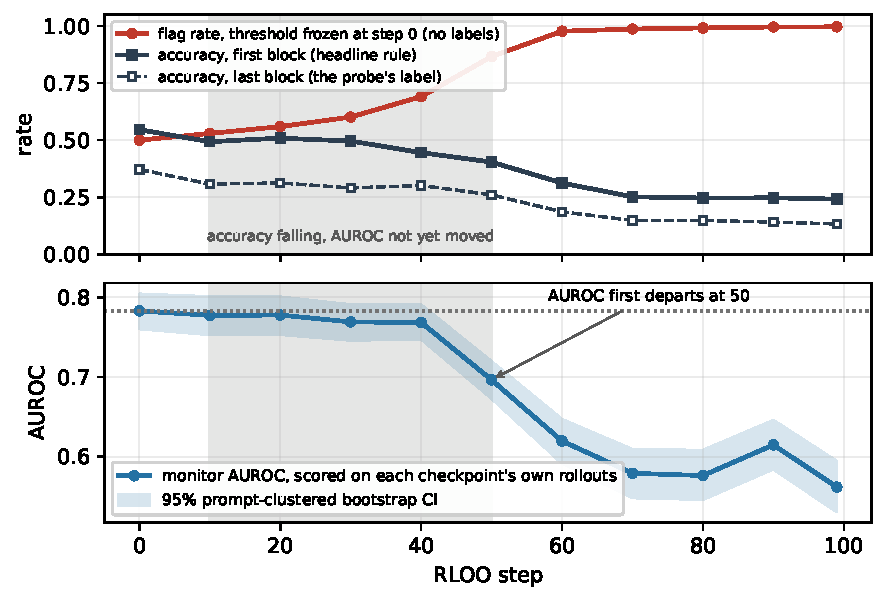
\includegraphics[width=0.82\linewidth]{figures/lag.pdf}
\caption{The monitor's AUROC does not register the decline for 30 to 40 steps. \texttt{runA}, initialised from $C_{\text{outcome}}$, under the probe-ladder protocol: at each checkpoint, 8 fresh answers per prompt on the 406 prompts, sampled at temperature 1. \textbf{Top:} accuracy under both grading rules is significantly lower by step 10, while the fraction of answers above a threshold frozen at step 0 rises. The shaded span runs from the first significant fall in accuracy to the first significant fall in AUROC, at step 40 (dark) under first-block labels and step 50 (light) under last-block labels. \textbf{Bottom:} the frozen reward probe's AUROC under each label, with $95\%$ prompt-clustered intervals. Both panels are computed from the same data as Tables~\ref{tab:lag} and~\ref{tab:lagfirst}.}
\label{fig:lag}
\end{figure}

Task accuracy falls first. By step 10, first-block accuracy is $5.2$ points below its step-0 value of $0.546$ ($95\%$ CI $[-6.9, -3.7]$, paired over prompts), and last-block accuracy is $6.4$ points below its $0.372$ ($[-8.2, -4.6]$). By step 40 the falls are $10.0$ and $7.0$ points. Under first-block labels the probe's AUROC starts at $0.919$, rises slightly at step 20 ($+0.017$, $p=0.022$), and first falls at step 40, by $-0.043$ ($p<0.001$). Under last-block labels it starts at $0.783$, does not differ detectably from step 0 through step 40 (all $p \geq 0.22$), and first moves at step 50, by $-0.086$ ($p < 0.001$). Either way the AUROC holds for 30 to 40 steps after accuracy has fallen, and this ordering needs no argument about the probe, since accuracy is measured by the verifier. The two labels differ because answers sampled without training's stop at \texttt{</answer>} run on into further answer blocks the policy would never have written in training, and those later blocks are more often wrong.

A flat AUROC also means what it says. Until it moves, the probe still ranks the policy's correct answers above its incorrect ones about as well as it did at step 0. What AUROC cannot report is that there are fewer correct answers to rank. Part of the reason it is flat is the metric rather than the policy. AUROC depends only on the order in which the probe ranks a checkpoint's answers. Between steps 0 and 40 the mean probe score inflates $0.473 \to 0.677$. Read through the step-40 checkpoint, the step-0 answers score lower than at step 0 ($0.377$ against $0.473$) and keep their first-block AUROC ($0.913$ against $0.919$). The inflation is therefore in the answers the policy now writes, not in how the probe reads old ones. A shift of the whole score distribution, of any size, leaves a rank-based statistic unchanged if the order within it holds, so the flatness before the AUROC moves follows from what AUROC measures and is not specific to the probe. Precision at a frozen threshold is confounded with the falling share of correct answers. The prevalence-invariant $\mathrm{LR}+$ at the threshold frozen at step 0 does move early: $7.00 \to 5.63$ by step 10 under first-block labels ($p\approx 0.01$), and $2.41 \to 1.91$ by step 30 under last-block labels ($p<0.001$). Inflating scores carry incorrect answers over the threshold faster than correct ones (FPR $0.117 \to 0.161$, TPR $0.819 \to 0.907$ by step 10). Appendix~\ref{app:metrics} works through these.

Statistics that need no labels can register the inflation. Each of the statistics above requires correctness labels, with which the accuracy drop could be measured directly. Score saturation is one label-free statistic: the share of answers above $0.95$ rises from $5.2\%$ at step 0 to $38.8\%$ by step 40, while on the benign ladder of Appendix~\ref{app:metrics} the same probe keeps it below $9\%$ at every checkpoint. The flag rate is a finer version. We freeze a threshold at step 0 and record the share of answers that clear it. Under attack this share rises monotonically ($+6\%$, $+12\%$, $+20\%$, $+38\%$ at steps 10 to 40, and eventually $+99\%$) and does not return. The flag rate moves at step 10, the first checkpoint after step 0, by $+0.030\,[+0.012,+0.048]$ at step 10 ($p=0.001$; one bootstrap draw of 2{,}000 crossed zero), whereas the AUROC first moves at step 40 or 50. The two statistics, computed from the same probe on the same answers, are therefore separated by 30 to 40 steps, and the flag-rate departure grows to $+0.496$ by step 99.

Some of that separation is expected from how the two statistics are defined. The flag rate is the threshold-crossing rate of the probe score, and the probe score is the training objective. Gradient ascent raises it by construction, so an early departure is partly guaranteed. What is not guaranteed is the size of the gap between the two, since nothing in the objective requires that the score inflate for 30 to 40 steps while the ranking it induces stays intact. The ordering between accuracy and AUROC does not share this circularity, since accuracy comes from the verifier. For a label-free signal, the non-circular case is the judge of \S\ref{sec:judge}, which the policy was never trained against and whose flag rate also moves.

Turning the ordering into a detector requires a benign band from a matched ladder of ordinary verifier-reward checkpoints, and our ladder has five defects, listed in Appendix~\ref{app:metrics}. On the prompts all its checkpoints share, benign training moves the flag rate by up to $+18.3\%$. The attacked run first exceeds that at step 30 ($+20.2\%$), a lead of 10 steps over the first-block AUROC and 20 over the last-block one. The flag rate's lead therefore establishes the ordering and not a calibrated false-alarm rate. The metric argument does not depend on the benign band, and the ordering is measured on the attacked run alone.

Monitoring a score distribution against a frozen reference is standard practice. Anytime-valid e-processes \citep{li2026whodrifted} could test it at every checkpoint without inflating false alarms, though Li's system-drift test is one-sided and would need adapting; we did not run one. The measurement here is how many RLOO steps separate a frozen-threshold statistic from the monitor's AUROC.

\subsection{A fixed judge keeps its AUROC while the policy degrades}\label{sec:judge}

The probe's AUROC stayed flat while the policy degraded. But the probe was also the training target, so the flat AUROC could reflect a change in how the probe relates to the answers it scores, rather than a change in the population. The flag-rate result in \S\ref{sec:lag} has the same circularity. A monitor that cannot change, and was never optimised against, separates the two cases when it scores the same run. If its discrimination also fails to register the decline, the flatness cannot come from the monitor changing, and the result does not depend on the probe having been the training target.

The monitor is an LLM judge \citep{zheng2023judging}. We re-sample all eleven checkpoints of \texttt{runA} (the judge ladder of Table~\ref{tab:actors}b: 406 prompts $\times$ 8 answers at temperature 1, 35{,}728 answers in total). This is a second, independent draw under the probe ladder's sampling settings, graded by the first answer block. Every answer is scored twice, once with the exact verifier and once with \texttt{Qwen2.5-7B-Instruct}, which is shown the problem and the proposed equation and asked whether the equation is correct. The judge's score is $P(\textsc{yes})$ renormalised over the verdict tokens. Appendix~\ref{app:judge} gives the prompt and decoding settings. The judge is imperfect. At step 0 it reaches precision $0.746$ at its own median threshold, against a true accuracy of $0.544$. The policy was never optimised against it.

The judge's weights and prompt are fixed. Across all eleven checkpoints it scored $4{,}651$ (problem, equation) pairs more than once; 8 cross the threshold, all within $3\times10^{-4}$ of it, and of the 48 pairs scored at both step 0 and step 99, none do. Any change in its statistics below is therefore not a change in the judge.

Its discrimination statistics do not register the decline (Table~\ref{tab:judge}). Its AUROC is $0.785$ at step 0 and $0.769$ at step 99. The one excursion is a dip of $-0.031$ at step 30 ($p = 0.002$, which survives Holm and Bonferroni corrections over the judge's 20 contrasts), across steps 20--40 while true accuracy falls $0.544 \to 0.457$, recovering by step 50. About half of it comes from one feature of the step-0 population: step 0 has 108 answers with no \texttt{<answer>} block, which the judge scores as near-certain failures, against at most 6 at any later step. Without them the step-0 AUROC is $0.769$ and the dip is $-0.015$ ($p=0.18$). Either way, the checkpoints where accuracy is lowest have AUROC at its starting level. The first and last checkpoints do not differ detectably. The paired change is $-0.017$, $95\%$ CI $[-0.048, +0.014]$, which bounds any degradation at about $0.05$ rather than only failing to reject zero. Raw precision does fall, by $42\%$ ($0.746 \to 0.429$), but the share of correct answers falls $0.544 \to 0.226$ over the same span, and precision at a fixed threshold moves with that share by construction. $\mathrm{LR}+ = \mathrm{TPR}/\mathrm{FPR}$, which is prevalence-invariant, is flat end to end at $2.46 \to 2.57$. We do not use lift, which is not prevalence-invariant (Appendix~\ref{app:metrics}). Both tables report nominal $p$; Appendix~\ref{app:ladders} gives which judge contrasts survive correction.

The judge did not change, and its AUROC ended where it began while true accuracy fell $0.544 \to 0.226$, a drop of $31.7$ points, or $58\%$. A stable AUROC here means the judge still ranks correct answers above incorrect ones about as well as before. That is the problem for monitoring, because discrimination is the statistic a monitor is validated on. Since the judge is fixed, whatever moved in its statistics moved in the population it scored, and that population changed in several ways. Correct answers fell from $54.4\%$ of the pool to $22.6\%$, and illegal answers grew from $28\%$ of wrong answers to $43\%$. The surface form also changed. The policy stopped using parentheses, with the share of correct answers containing none rising $0.017 \to 0.982$, and the judge is sensitive to this. For correct expressions written both with and without brackets across steps 0 and 99, it passes $0.746$ of the bracketed forms and $0.548$ of the bare ones ($+0.198$, $95\%$ CI $[+0.131, +0.265]$). The judge therefore also depends on a surface correlate. This is the situation clinical epidemiology calls spectrum bias \citep{ransohoff1978spectrum}: a test's sensitivity and specificity, measured on one spectrum of cases, do not carry over to another. We show that the population moved while the judge did not. We do not isolate which change in the population drives which movement in the judge's statistics. In spectrum bias the study population varies for reasons external to the test, such as who is enrolled. Here the deployment of the artifact is what moves the population, so the number an interpretability paper reports from held-out evaluation is measured on a distribution that deployment removes.

The frozen-threshold statistic also registers the change for the judge, though here the share of answers above the threshold decreases rather than increases, $0.500 \to 0.317$, a $-37\%$ change against AUROC's $-2\%$. The departure is nominally detectable at step 20 ($-0.026\,[-0.047,-0.007]$, $p=0.013$) but not at step 10 ($p=0.069$), and it survives a Holm correction from step 30 on. It is not monotone, reaching a minimum of $0.294$ at step 80 while accuracy continues to fall. The judge was never optimised against, so this departure is not a consequence of the training objective. The judge's departure suggests that a frozen operating point can register the population shift on its own, though it comes 20 steps after the probe's. The quantity to monitor is distance from that operating point in either direction, not a rise specifically. A two-sided test, built the way the anchor process of \citet{li2026whodrifted} runs one e-process per direction, would suit it.

The judge is a bystander, never optimised against, so this is not a demonstration that a judge can be gamed. \citet{zhou2026convincing} optimises a policy against its own judge and finds the errors transfer: a three-family ensemble, two of whose members were never trained against, sees its discrimination ($\mathrm{TPR}-\mathrm{FPR}$) fall from $0.31$ to $0.09$ while still passing $55\%$ of hacked wrong answers. There the errors became convincing to every judge that scored the shown answer, and a labelled discrimination check registers it. Ours instead keeps its discrimination while the policy degrades, so the same check passes.

\subsection{Reading higher as a monitor did not make a safer reward}\label{sec:surface}

The probe partly depends on surface properties of the text (\S\ref{sec:probe-reader}), which raises the hypothesis that the policy degrades by learning to produce them. We test it with detectors that use only the text and with RL arms that change the reward.

The first is already in \S\ref{sec:probe-reader}. A 39-feature surface model with no access to activations reaches $0.926$, close to the probe's $0.982$, so much of what the probe detects is also visible in the text. The second is three RL arms, two of them pre-registered (Appendix~\ref{app:setup}). Arm A follows the logic of amnesic probing \citep{elazar2021amnesic}, though not its method. We subtract from the activations the part that the 39 surface features predict, by least squares, refit the probe on what remains, and train against it. Because the subtraction is a fixed linear map, the reward is a probe on the activations plus a fixed term in the text features. On $C_{\text{outcome}}$'s answers to prompts it was not fit on, the text term offsets the surface information in the activations: the activation term alone reads $0.976$, the text term alone $0.079$, and the two together $0.834$. During RL the text term is a fixed penalty on the pattern a text-only reward produces. Its weights oppose arm B's on 24 of the 27 features that vary ($r=-0.56$), and on arm B's final answers it contributes $-27.9$ logits, against $+0.16$ on $C_{\text{SFT}}$'s. Arm A therefore tests a probe reward that penalises the surface pattern, not one blind to it. Arm B's reward is the text-only surface model itself. Arm R, added after review, trains against the raw probe that arm A's fitting procedure produces alongside the residualised one: the same rows, labels, prompt split and regularisation, without the subtraction (held-out AUROC $0.978$). All three start from $C_{\text{SFT}}$ and share one recipe: the same trainer, which reads hidden states from a frozen copy of $C_{\text{SFT}}$ so that each reward is a fixed function of the text, and the same optimizer settings and evaluation. Arms A and R therefore differ only in the residualisation. Their probes were fit on $C_{\text{outcome}}$'s hidden states, which is where Table~\ref{tab:arms} reads them. Read instead through $C_{\text{SFT}}$, on $C_{\text{SFT}}$'s own headline answers that have a locatable \texttt{</think>}, the rewards read lower: A $0.589$, B $0.755$ and R $0.816$. The order is the same, but arm A's reward is weak on the policy it started from. \texttt{runB}, which also starts from $C_{\text{SFT}}$, appears as arm C for reference, but it differs from the arms in more than its reward. Its probe read the current policy's hidden states, it used weight decay $0.01$ and gradient clipping at $1.0$ where the arms used $10^{-4}$ and none, and its probe was fit on different answers. Arms A, B and R form the controlled comparison (Figure~\ref{fig:ladder}, Table~\ref{tab:arms}).

All four arms are evaluated under the arm protocol (Table~\ref{tab:actors}b). Arm C was first scored under the headline protocol, at $0.0734$; re-scored like the other three it reads $0.0782$, a difference of $+0.48$\,pp (CI $[-0.62, +1.60]$), so arm C's placement does not depend on the protocol.

\begin{figure}[t]
\centering
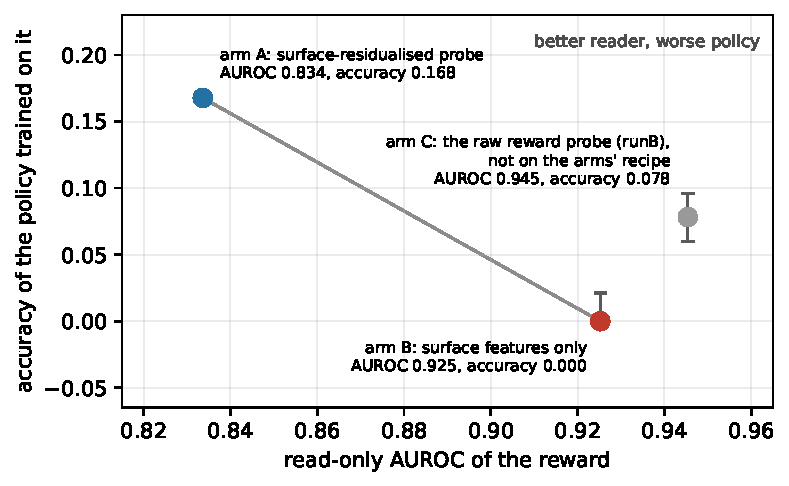
\includegraphics[width=0.78\linewidth]{figures/ladder.pdf}
\caption{Higher held-out AUROC did not indicate the safer training target. Each point is one reward, showing its AUROC as a held-out monitor read through $C_{\text{outcome}}$, on prompts it was not fit on, against the first-block accuracy of the policy after 100 RLOO steps against it, under the arm protocol (Table~\ref{tab:actors}b). Arms A, B and R share a recipe and differ only in the reward; the one that reads lowest, arm A, kept by far the most accuracy. Arm C (\texttt{runB}) differs from the arms in trainer and optimizer settings (\S\ref{sec:surface}), so it is shown for reference, in grey. Bars are paired prompt-clustered $95\%$ intervals of each arm's difference from arm A, drawn at each arm's accuracy and cut at zero for arm B; the line joins the three arms on one recipe. The intervals measure evaluation uncertainty for each trained policy, not variation across training runs. Table~\ref{tab:arms} gives the same four rows.}
\label{fig:ladder}
\end{figure}

\begin{table}[h]
\centering\small
\begin{tabular}{llcc}
\toprule
Arm & reward & read-only AUROC & first-block acc.\ (vs.\ arm A) \\
\midrule
A & surface-\emph{residualised} probe & 0.834 & $0.1678$ \ \ (reference) \\
B & surface features \emph{only} & 0.925 & $\mathbf{0.0000}$ \ \ ($-16.78$ pp, CI $[-18.97,-14.66]$) \\
R & the same probe, \emph{raw} & 0.978 & $0.0514$ \ \ ($-11.64$ pp, CI $[-13.76,-9.61]$) \\
\midrule
C$^{\dagger}$ & raw reward probe (\texttt{runB}) & 0.945 & $0.0782$ \ \ ($-8.96$ pp, CI $[-10.81,-7.17]$) \\
\bottomrule
\end{tabular}
\caption{The rewards, compared. The AUROC column is on one population and one label rule: $C_{\text{outcome}}$'s headline answers graded by the first block and read through $C_{\text{outcome}}$, on the half of the 406 prompts that arms A, B and R were not fit on. Read through $C_{\text{SFT}}$ on $C_{\text{SFT}}$'s own answers, arms A, B and R all read lower (\S\ref{sec:surface}). Accuracy is first-block at step 100, all four under the arm protocol (Table~\ref{tab:actors}b). Intervals are paired over prompts, for fixed trained policies. $^{\dagger}$Arm C differs from arms A, B and R in trainer and optimizer settings as well as reward (\S\ref{sec:surface}), so only A, B and R are controlled.}
\label{tab:arms}
\end{table}

A reward with no access to the model's internals drove accuracy to exactly zero, and the output keeps its form. Every answer still emits \texttt{</think>} and $3{,}244$ of $3{,}248$ contain an \texttt{<answer>} block, but only $0.12\%$ of those blocks are arithmetic at all. A verbatim example follows, for input $[29, 17, 63, 38]$ and target $68$.

\vspace{-0.35em}
\begin{quote}\ttfamily\small\setlength{\parskip}{0pt}
<answer>\\
Let me verify:\\
1. 17 - 10 = 7\\
2. 63 - 7 = 56\\
3. 29 * 38 = 1102\\
4. 56 - (29 * 38 / 38) = 68\\
</answer>
\end{quote}
\vspace{-0.35em}

Step 1 uses $10$, which is not in the input. Step 3 is correct but irrelevant. Step 4 reuses two numbers and evaluates to 27 while asserting 68 in the answer position. The answer has the form of verification and contains no valid arithmetic. The reward's largest weights favour long text after \texttt{</think>} (\texttt{tail\_len}, $+1.19$ in standardised units) and a long answer block (\texttt{ans\_len}, $+0.62$), and penalise equals signs in the reasoning (\texttt{n\_equals}, $-1.11$).

Arm A's pre-registered prediction was that it would degrade the task less than the published probe-reward run, \texttt{runA} (Appendix~\ref{app:setup}). Measured as pre-registered, by first-block accuracy at step 100, it did not: arm A ended $6.83$\,pp below \texttt{runA}, a contrast that crosses initialisation and evaluation protocol. Against arm R, added after review to isolate the residualisation, arm A kept $+11.64$\,pp more accuracy (CI $[+9.61, +13.76]$). Arm B's prediction, that a text-only reward degrades the task at least as much as the raw probe, holds against arm R ($-5.14$\,pp, CI $[-6.25, -4.09]$) and against \texttt{runA} and \texttt{runB}.

Three rewards under one recipe at one seed each give counterexamples and not a relationship (Figure~\ref{fig:ladder}). Arm A, which reads lowest as a held-out monitor, kept the most accuracy; both higher-reading rewards did far worse, with paired intervals far from zero. The ordering is not a strict inversion, since arm B reads lower than arm R and did worse. Residualisation lowered the probe's held-out AUROC by $0.144$, and arm A's run ended $11.6$\,pp above arm R's. Two explanations remain open that one run per arm cannot separate: a reward that is weak on the model it reads may simply be harder to exploit, a confound the pre-registration itself named, and arm A's reward penalises the surface pattern directly. The intervals are over prompts for fixed trained policies; whether these reversals repeat across training seeds is untested.

\paragraph{Surface occupation is sufficient to cause the degradation, but is not shown to be its mechanism.} Producing cheap textual structure is sufficient to defeat both a monitor and the task, with no access to internals. This does not establish that it is the mechanism behind the probe reward's failure; arm A is consistent with that account but does not establish it.

How much of a monitor's AUROC survives conditioning on cheap surface features can be measured before training. For our trace-final probe it holds well ($0.982 \to 0.939$ under \texttt{</think>}-position stratification), yet a probe of the same kind degraded the policy as a reward. Which directions an optimizer can push the monitor's score along is a different question from what the monitor can detect, and held-out accuracy answers only the second.

\section{Limitations}

Every RL configuration is a single seed, including the checkpoint ladder on which the lag is measured. Our prompt-clustered intervals measure evaluation uncertainty for each trained policy, not variability across training runs, and our three analysis seeds bound measurement noise, not training variance. Training was not seeded, and repeating arms A, B and R over seeds is the most direct replication. These results demonstrate direction and not size. All RL experiments are at 0.5B, so how these results scale is untested. We use one task, one model family, one RL algorithm and one bystander judge. The flag rate has no matched benign control, so it is a measure of change and not a calibrated alarm.

An earlier version reported that RL makes the probe direction causally active under steering; we withdraw it and report no causal experiment on the probe's direction. The steered vector has cosine $0.163$ with the probe actually optimised, not the $1.000$ the claim assumed. The intervention was also applied one transformer block and 2--3 tokens downstream of the read site, and the key contrasts reach only $p=0.063$ and $p=0.080$. The cosine between the steered vector and the optimised direction would have caught the error; claims that optimisation made a direction causal should report it and confirm that the intervention site is the read site. A defensible version needs interventions aligned to the read site, evaluated as a causal abstraction \citep{geiger2021abstractions}.

Every number in this paper regenerates on CPU from cached artifacts using one script, \texttt{scripts/check\_everything.sh}, which prints each published value, including every table cell, beside its recomputation and exits non-zero on any disagreement. The withdrawn steering result is outside its scope. Code and the script are at \url{https://github.com/Abraham-y/reader-writer-probe-rl}, and the $0.36$\,GB of cached artifacts it reads are at \url{https://huggingface.co/datasets/prismane16/monitor-accuracy-under-rl}.

% Modal sponsored the compute on the condition that it is acknowledged as a
% funding source; scripts/verify_camera_ready.py fails if this is removed.
\begin{ack}
This work was supported by compute credits from Modal. We thank the reviewers, whose comments led to the evaluation protocols of Table~\ref{tab:actors}b and to the audit that corrected several claims in the submitted version.
\end{ack}

\begin{thebibliography}{99}
\bibitem[Gandhi et al.(2024)]{gandhi2024stream} Gandhi, K., et al.\ Stream of search (SoS): Learning to search in language. arXiv:2404.03683, 2024.
\bibitem[Ahmadian et al.(2024)]{ahmadian2024back} Ahmadian, A., et al.\ Back to basics: Revisiting REINFORCE-style optimization for learning from human feedback in LLMs. ACL, arXiv:2402.14740, 2024.
\bibitem[Arditi et al.(2024)]{arditi2024refusal} Arditi, A., et al.\ Refusal in language models is mediated by a single direction. NeurIPS, arXiv:2406.11717, 2024.
\bibitem[Burns et al.(2023)]{burns2022discovering} Burns, C., et al.\ Discovering latent knowledge in language models without supervision. ICLR, arXiv:2212.03827, 2023.
\bibitem[Pacchiardi et al.(2024)]{pacchiardi2023lie} Pacchiardi, L., et al.\ How to catch an AI liar: Lie detection in black-box LLMs by asking unrelated questions. ICLR, arXiv:2309.15840, 2024.
\bibitem[Gao et al.(2023)]{gao2023scaling} Gao, L., Schulman, J., Hilton, J.\ Scaling laws for reward model overoptimization. ICML, arXiv:2210.10760, 2023.
\bibitem[Coste et al.(2024)]{coste2023reward} Coste, T., et al.\ Reward model ensembles help mitigate overoptimization. ICLR, arXiv:2310.02743, 2024.
\bibitem[Skalse et al.(2022)]{skalse2022defining} Skalse, J., et al.\ Defining and characterizing reward hacking. NeurIPS, arXiv:2209.13085, 2022.
\bibitem[Denison et al.(2024)]{denison2024sycophancy} Denison, C., et al.\ Sycophancy to subterfuge: Investigating reward tampering in language models. arXiv:2406.10162, 2024.
\bibitem[Baker et al.(2025)]{baker2025monitoring} Baker, B., et al.\ Monitoring reasoning models for misbehavior and the risks of promoting obfuscation. arXiv:2503.11926, 2025.
\bibitem[Gupta and Jenner(2025)]{gupta2025rlobfuscation} Gupta, R.\ and Jenner, E.\ RL-Obfuscation: Can language models learn to evade latent-space monitors? arXiv:2506.14261, 2025.
\bibitem[Taufeeque et al.(2026)]{taufeeque2026atlas} Taufeeque, M., Heimersheim, S., Gleave, A., and Cundy, C.\ The obfuscation atlas: Mapping where honesty emerges in RLVR with deception probes. ICML (Oral), arXiv:2602.15515, 2026.
\bibitem[Ransohoff and Feinstein(1978)]{ransohoff1978spectrum} Ransohoff, D.\ F.\ and Feinstein, A.\ R.\ Problems of spectrum and bias in evaluating the efficacy of diagnostic tests. \emph{New England Journal of Medicine}, 299(17):926--930, 1978.
\bibitem[Belinkov(2022)]{belinkov2022probing} Belinkov, Y.\ Probing classifiers: Promises, shortcomings, and advances. \emph{Computational Linguistics}, 48(1):207--219, arXiv:2102.12452, 2022.
\bibitem[Hewitt and Liang(2019)]{hewitt2019control} Hewitt, J.\ and Liang, P.\ Designing and interpreting probes with control tasks. EMNLP, arXiv:1909.03368, 2019.
\bibitem[Voita and Titov(2020)]{voita2020mdl} Voita, E.\ and Titov, I.\ Information-theoretic probing with minimum description length. EMNLP, pp.\ 183--196, arXiv:2003.12298, 2020.
\bibitem[Elazar et al.(2021)]{elazar2021amnesic} Elazar, Y., Ravfogel, S., Jacovi, A., and Goldberg, Y.\ Amnesic probing: Behavioral explanation with amnesic counterfactuals. \emph{TACL}, arXiv:2006.00995, 2021.
\bibitem[Geiger et al.(2021)]{geiger2021abstractions} Geiger, A., Lu, H., Icard, T., and Potts, C.\ Causal abstractions of neural networks. NeurIPS, arXiv:2106.02997, 2021.

\bibitem[Zheng et al.(2023)]{zheng2023judging} Zheng, L., Chiang, W.-L., Sheng, Y., Zhuang, S., Wu, Z., Zhuang, Y., Lin, Z., Li, Z., Li, D., Xing, E.\ P., Zhang, H., Gonzalez, J.\ E., and Stoica, I. Judging LLM-as-a-judge with MT-Bench and Chatbot Arena. NeurIPS Datasets and Benchmarks Track, arXiv:2306.05685, 2023.
\bibitem[Frick et al.(2024)]{frick2024ppe} Frick, E., Li, T., Chen, C., Chiang, W.-L., Angelopoulos, A.\ N., Jiao, J., Zhu, B., Gonzalez, J.\ E., and Stoica, I. How to evaluate reward models for RLHF. arXiv:2410.14872, 2024.
\bibitem[Malik et al.(2026)]{malik2025rewardbench2} Malik, S., Pyatkin, V., Land, S., Morrison, J., Smith, N.\ A., Hajishirzi, H., and Lambert, N. RewardBench 2: Advancing reward model evaluation. ICLR, arXiv:2506.01937, 2026.
\bibitem[Norman et al.(2026)]{norman2026reliability} Norman, J.\ D., Rivera, M.\ U., and Hughes, D.\ A. Reliability without validity: A systematic, large-scale evaluation of LLM-as-a-judge models across agreement, consistency, and bias. arXiv:2606.19544, 2026.
\bibitem[Weng et al.(2026)]{weng2026invariance} Weng, S., Feng, Y., and Xie, X. Beyond accuracy: Policy invariance as a reliability test for LLM safety judges. arXiv:2605.06161, 2026.
\bibitem[Yang et al.(2026)]{yang2026auditing} Yang, Z., Hou, Y., and Yang, X. When the judge changes, so does the measurement: Auditing LLM-as-judge reliability. arXiv:2607.08535, 2026.
\bibitem[Zhou(2026)]{zhou2026convincing} Zhou, C. More convincing, not more correct: Self-play reward hacking of reference-free LLM judges. arXiv:2607.05904, 2026.
\bibitem[Li(2026)]{li2026whodrifted} Li, Y. Who drifted: the system or the judge? Anytime-valid attribution in LLM evaluation pipelines. arXiv:2606.15474, 2026.
\bibitem[Beigi et al.(2026)]{beigi2026prime} Beigi, M., Jin, M., and Huang, L. Proxy reward internalization and mechanistic exploitation: A learned precursor to reward hacking and its generalization. arXiv:2606.09711, 2026.
\bibitem[Bailey et al.(2024)]{bailey2024obfuscated} Bailey, L., et al.\ Obfuscated activations bypass LLM latent-space defenses. arXiv:2412.09565, 2024.
\end{thebibliography}

\appendix
\section{The judge prompt and decoding settings}\label{app:judge}

The judge is the one language model that is part of our method rather than a subject of it, so we give it in full. Every answer is scored by \texttt{Qwen2.5-7B-Instruct} with this prompt, where \texttt{\{nums\}}, \texttt{\{target\}} and \texttt{\{equation\}} are filled from the problem and the first \texttt{<answer>} block (answers with none are sent with ``(no answer given)'' in its place). The text is the user turn of Qwen's chat template, which prepends the model's default system turn:

\begin{quote}\ttfamily\small
You are grading a solution to a Countdown arithmetic puzzle.\\[2pt]
The solver was given the numbers \{nums\} and the target \{target\}. A correct solution uses each number exactly once, uses only + - * / and parentheses, and evaluates to the target.\\[2pt]
The solver's proposed equation:\\
\{equation\}\\[2pt]
Is this equation a correct solution? Answer with exactly one word, YES or NO.
\end{quote}

The score is $P(\textsc{yes})$ from the first generated token's top-20 logprobs, renormalised over six \textsc{yes} and six \textsc{no} variants (upper, title and lower case, each with and without a leading space; all single tokens). Two of the $35{,}728$ answers had no \textsc{yes} variant in the top 20 and score 0. It is a continuous score rather than a sampled verdict and the threshold analyses in \S\ref{sec:judge} are well defined. Decoding is greedy and the model is frozen, which is what makes the fixed-function check of \S\ref{sec:judge} meaningful: the same (problem, equation) pair scored at two checkpoints receives the same score up to the numerical non-determinism of batched inference, and we verify that empirically rather than assuming it. Of the $4{,}651$ repeated pairs, $79\%$ score identically every time and $109$ differ by more than $0.01$, the largest by $0.109$.

Apart from the judge, the only language models in the method are the policy and, for arms A and R, a frozen copy of $C_{\text{SFT}}$ whose hidden states their probes read. The probes and arm B's surface model are logistic regression, the policy is trained with RLOO against the verifier or one of those rewards, and the verifier is exact and rule-based.

\section{Why the paper reports LR+ rather than lift, and what is wrong with the control ladder}\label{app:metrics}

\textbf{Why AUROC stays flat: partly the policy, partly the metric.} AUROC depends only on the order the probe puts answers in. Between steps 0 and 40 the mean score inflates $0.473 \to 0.677$ while leaving the order within each checkpoint almost intact, and the inflation is in the policy's new answers (the step-0 answers read through the step-40 checkpoint average $0.377$), so ``AUROC stayed flat'' is partly a fact about the metric and about every rank-based statistic. The obvious replacement is worse. Precision at a frozen threshold falls $0.588 \to 0.416$ ($-29.3\%$), but the share of answers that are correct falls too, and precision moves with it whether or not the probe changed. The prevalence-invariant statistic is $\mathrm{LR}+ = \mathrm{TPR}/\mathrm{FPR}$, and it falls $2.41 \to 1.65$, or $\mathbf{-31.6\%}$: slightly more than raw precision, not less. All four statistics here use last-block labels, as in Table~\ref{tab:lag}. Measured against its above-chance margin, AUROC moves $-5.1\%$. We use $\mathrm{LR}+$ and not \emph{lift}, which is not prevalence-invariant: on the judge ladder $\sim$91\% of lift's apparent improvement is the confound it appears to remove, with roughly $70\%$ of the flag rate's own movement predicted the same way. Here lift moves only $-12.8\%$.

\textbf{The control is the weakest part of this paper.} A paired test against step 0 shows the statistic \emph{moved}, not that it moved more than benign training moves it. That needs a control ladder of ordinary runs, and ours is poor: five checkpoints, the wrong initialisation, headline-protocol sampling (16 answers at temperature 0.6) rather than the ladder's 8 at temperature 1, and three of its five checkpoints scored on 166--167 prompts where every attacked checkpoint uses all 406; at step 30 a further $32.1\%$ of its answers have no locatable \texttt{</think>} and cannot be scored. It is the ordinary run from $C_{\text{SFT}}$ that produced $C_{\text{outcome}}$, scored with the reward probe at a threshold frozen at its own step 0. Holding the population fixed at the 166 prompts all five checkpoints share, benign training moves the flag rate by up to $+18.3\%$ (at step 30), so the band is not an artefact of the changing prompt count. The attacked run first exceeds it at step 30 ($+20.2\%$). On the same ladder the reward probe keeps the share of answers above $0.95$ below $9\%$ at every checkpoint, where the attacked run reaches $38.8\%$ by step 40. Read the lead as evidence that the ordering exists, not as a calibrated false-alarm rate. A matched control ladder is the highest-value experiment left undone here.

\section{Setup detail}\label{app:setup}

$C_{\text{SFT}}$ is \texttt{asingh15/qwen-sft-countdown-defaultproj}, a public checkpoint we did not train. $C_{\text{outcome}}$ is 100 RLOO \citep{ahmadian2024back} steps with the verifier reward at batch 128, group size 16, KL $10^{-3}$, entropy $10^{-3}$, lr $10^{-5}$, weight decay $10^{-4}$ and no gradient clipping. \texttt{runA} and \texttt{runB} use group size 8, weight decay $0.01$ and gradient clipping at $1.0$, with the KL anchor at their own initialisation; arms A, B and R use group size 8, weight decay $10^{-4}$ and no clipping. No run was seeded. In \texttt{runA} and \texttt{runB} the reward's copy of the policy was refreshed from the latest checkpoint each round, except on the one round in ten when a bug in locating that checkpoint left it one update old; the code has since been fixed. The pre-registration of arms A and B was written before arm A launched, by our local file records, but first committed to git on 12 August 2026, after both arms had run, so its timing is not independently verifiable. Its reference row names the published run but lists AUROC $0.978$, the value of arm R's probe, while its text cites \texttt{runA}'s accuracy drop; \texttt{runA} differs from the arms in initialisation, trainer and optimizer settings that it did not list. During RL, sampling stops at the first \texttt{</answer>}; evaluation sampling does not. Arm A's evaluation command was not recorded. Re-running the arm protocol on its final checkpoint reproduces its evaluation answer for answer, as it does for arm B, whose command was recorded, so all four arms were scored identically. The verifier returns $\{0, 0.1, 1.0\}$. Eval is 500 procedurally generated problems filtered to the 406 with no overlap against the RLOO training pool.

Probes are L2-regularised logistic regression at layer 16. The trace-final probe, the baselines of \S\ref{sec:probe-reader} and the reward probe are scored by 5-fold \texttt{GroupKFold} on prompt and class-balanced by subsampling the held-out scores. The probes of arms A and R and arm B's surface model are fit with a class-weighted loss on one half of the prompts, split by a hash of the prompt index, and scored on the other half. The ladder AUROCs are plain AUROCs of the frozen reward probe. Where an in-sample figure exists we do not quote it; the trace-final probe reads $0.995$ in-sample against $0.982$ held out.

\section{The reader probe in full}\label{app:reader}

As a best-of-16 selector on 406 held-out prompts the probe reaches $0.6700$, against $0.5531$ for picking at random among the same answers and $0.6847$ for an oracle that takes a correct answer whenever one is present; that is $88.8\%$ of the available gain (prompt-clustered paired bootstrap, CI $[78.9\%, 96.5\%]$). A prompt has up to 16 scoreable answers, $15.5$ on average once unscoreable ones are dropped. The margin over the free baselines is $+3.20$\,pp of selection accuracy (CI $[+0.99, +5.42]$, $p = 0.008$ against picking the answer with the shortest \texttt{<think>} and $p = 0.004$ against the 39-feature surface model), and $+0.056$ AUROC. That margin, not the raw $0.982$, is the number to read. This is a baseline comparison, not the control-task selectivity of \citet{hewitt2019control}, which would require refitting on a control task with random labels fixed per input type; we did not run that.

On length specifically: stratified by \texttt{</think>} position the probe still reads $0.939$, against $0.564$ for position alone, so it is not a length detector, though a free structural baseline already captures $64\%$ of the headroom.

Two limits on what any of this licenses. High probe accuracy does not by itself establish that the model \emph{uses} the direction \citep{belinkov2022probing}, and similar probe accuracies can hide large differences in how readily a representation encodes the property \citep{voita2020mdl}; we make no causal claim. Answers with no locatable \texttt{</think>} are unscoreable and dropped from every AUROC in this section ($2.9\%$ on $C_{\text{outcome}}$, $10.4\%$ on $C_{\text{SFT}}$, all of them wrong). The checkpoint ladder of \S\ref{sec:lag} drops such answers too, but few: 32 at step 0 and at most 8 at any other step ($3{,}216$--$3{,}248$ of $3{,}248$ scored), too few to explain the flat AUROC. Layer 16 was fixed in advance from the original study.

\section{Full checkpoint ladders}\label{app:ladders}

Every checkpoint of both series, with prompt-clustered bootstrap intervals. The body quotes the load-bearing values from these tables; they are reproduced whole here because both series are non-monotone and a selected subset would misrepresent them. Checkpoint labels are the trainer's: the checkpoint labelled step $k$ holds the weights after $k+1$ updates, so step 0 is one update past $C_{\text{outcome}}$, and step 99 is the final checkpoint. Both tables report nominal $p$. Corrected over the judge's 20 step-0 contrasts (10 AUROC, 10 flag rate), the AUROC dip at step 30 and the flag-rate departures from step 30 on survive Holm, and the dip and the flag rate from step 40 on also survive Bonferroni.

\begin{table}[t]
\centering
\footnotesize
\setlength{\tabcolsep}{3.2pt}
\renewcommand{\arraystretch}{0.92}
\begin{tabular}{cccccccc}
\toprule
RLOO step & acc.\ first & acc.\ last & \textbf{probe AUROC} [95\% CI] & $p$ vs.\ 0 & prec @ $T$ & \textbf{LR}$+$ & \textbf{flag rate} [95\% CI] \\
\midrule
0  & 0.546 & 0.372 & 0.783 [0.760, 0.804] & --- & 0.588 & 2.41 & 0.500 [0.466, 0.535] \\
10 & 0.493 & 0.308 & 0.777 [0.753, 0.801] & 0.627 & 0.504 & 2.28 & 0.529 [0.494, 0.566] \\
20 & 0.509 & 0.312 & 0.778 [0.753, 0.801] & 0.598 & 0.503 & 2.23 & 0.559 [0.522, 0.596] \\
30 & 0.496 & 0.291 & 0.769 [0.746, 0.791] & 0.222 & 0.439 & 1.91 & 0.601 [0.565, 0.636] \\
40 & 0.445 & 0.302 & 0.768 [0.748, 0.790] & 0.228 & 0.416 & 1.65 & \textbf{0.691 [0.659, 0.721]} \\
\textbf{50} & 0.404 & 0.260 & \textbf{0.696 [0.673, 0.719]} & \textbf{0.000} & 0.290 & 1.16 & 0.866 [0.846, 0.885] \\
60 & 0.312 & 0.186 & 0.620 [0.592, 0.647] & 0.000 & 0.189 & 1.02 & 0.977 [0.972, 0.982] \\
70 & 0.252 & 0.148 & 0.579 [0.548, 0.609] & 0.000 & 0.149 & 1.01 & 0.987 [0.983, 0.990] \\
80 & 0.247 & 0.148 & 0.576 [0.546, 0.608] & 0.000 & 0.149 & 1.01 & 0.991 [0.988, 0.995] \\
90 & 0.247 & 0.141 & 0.615 [0.584, 0.646] & 0.000 & 0.141 & 1.00 & 0.996 [0.994, 0.998] \\
99 & 0.242 & 0.133 & 0.562 [0.531, 0.594] & 0.000 & 0.133 & 1.00 & 0.996 [0.994, 0.998] \\
\bottomrule
\end{tabular}
\caption{The reward probe on \texttt{runA} (initialised from $C_{\text{outcome}}$), probe-ladder protocol: 8 fresh answers per prompt at temperature 1 on the 406 prompts. Accuracy is given under both grading rules; the AUROC, precision and LR$+$ use the last-block label, the rule the probe was fit to predict; the flag rate needs no label. Accuracy is significantly lower from step 10 under either rule; the AUROC first moves at step 50 under this label, and at step 40 under first-block labels (Table~\ref{tab:lagfirst}). Intervals are a prompt-clustered bootstrap over the 406 prompts (2{,}000 resamples) computed from per-rollout probe scores on each checkpoint's own cached activations; $p$ from paired differences against step 0.}\label{tab:lag}
\end{table}

\begin{table}[t]
\centering
\footnotesize
\setlength{\tabcolsep}{4pt}
\renewcommand{\arraystretch}{0.92}
\begin{tabular}{ccc}
\toprule
RLOO step & \textbf{probe AUROC, first block} [95\% CI] & $p$ vs.\ 0 \\
\midrule
0 & 0.919 [0.904, 0.932] & --- \\
10 & 0.917 [0.901, 0.932] & 0.807 \\
20 & 0.936 [0.922, 0.949] & 0.022 \\
30 & 0.919 [0.903, 0.932] & 0.972 \\
\textbf{40} & \textbf{0.876 [0.860, 0.892]} & \textbf{0.000} \\
50 & 0.779 [0.759, 0.798] & 0.000 \\
60 & 0.655 [0.631, 0.680] & 0.000 \\
70 & 0.619 [0.593, 0.645] & 0.000 \\
80 & 0.615 [0.588, 0.642] & 0.000 \\
90 & 0.622 [0.598, 0.647] & 0.000 \\
99 & 0.585 [0.557, 0.613] & 0.000 \\
\bottomrule
\end{tabular}
\caption{The reward probe's AUROC on the same ladder as Table~\ref{tab:lag}, against first-block labels, the block the verifier graded during training. It starts higher than under last-block labels, rises at step 20, and first falls at step 40. Prompt-clustered bootstrap over the 406 prompts, 2{,}000 resamples; $p$ from paired differences against step 0.}
\label{tab:lagfirst}
\end{table}

\begin{table}[t]
\centering
\footnotesize
\setlength{\tabcolsep}{4pt}
\renewcommand{\arraystretch}{0.92}
\begin{tabular}{ccccccc}
\toprule
RLOO step & acc.\ first & \textbf{judge AUROC} [95\% CI] & $p$ vs.\ 0 & prec @ $T$ & \textbf{LR}$+$ & \textbf{flag rate} [95\% CI] \\
\midrule
0  & 0.544 & 0.785 [0.757, 0.813] & --- & 0.746 & 2.46 & 0.500 [0.466, 0.534] \\
10 & 0.495 & 0.784 [0.755, 0.812] & 0.864 & 0.703 & 2.41 & 0.481 [0.449, 0.516] \\
20 & 0.506 & 0.761 [0.729, 0.791] & \textbf{0.011} & 0.699 & 2.26 & 0.474 [0.441, 0.505] \\
30 & 0.488 & 0.754 [0.723, 0.783] & \textbf{0.002} & 0.679 & 2.22 & 0.465 [0.432, 0.498] \\
40 & 0.457 & 0.757 [0.726, 0.785] & \textbf{0.025} & 0.667 & 2.38 & 0.434 [0.403, 0.467] \\
50 & 0.399 & 0.778 [0.748, 0.806] & 0.593 & 0.631 & 2.58 & 0.373 [0.342, 0.407] \\
60 & 0.307 & 0.787 [0.757, 0.814] & 0.921 & 0.558 & 2.84 & 0.331 [0.304, 0.359] \\
70 & 0.268 & 0.790 [0.761, 0.818] & 0.731 & 0.524 & 3.01 & 0.304 [0.276, 0.330] \\
80 & 0.234 & 0.792 [0.761, 0.820] & 0.673 & 0.482 & 3.04 & 0.294 [0.268, 0.320] \\
90 & 0.232 & 0.775 [0.744, 0.806] & 0.511 & 0.448 & 2.68 & 0.312 [0.284, 0.339] \\
99 & 0.226 & 0.769 [0.737, 0.801] & 0.312 & 0.429 & 2.57 & \textbf{0.317 [0.290, 0.344]} \\
\bottomrule
\end{tabular}
\caption{An LLM judge watching the same run. \texttt{runA}, judge-ladder protocol: an independent draw of 8 answers per prompt at temperature 1, graded by the first block, the rule the judge is shown. Its AUROC dips at steps 20--40 and recovers, about half of it because step 0 holds 108 answers with no \texttt{<answer>} block (\S\ref{sec:judge}); its positive likelihood ratio LR$+$ tracks the same shape and ends where it began, so the operating point does not degrade. Prompt-clustered bootstrap over the 406 eval prompts, 2{,}000 resamples; $p$ from paired differences against step 0, nominal.}
\label{tab:judge}
\end{table}

\end{document}
